%%%% main.tex, 2022/08/10, 2.5
%%%% Copyright (C) 2020 Vinicius Pegorini (vinicius@utfpr.edu.br)
%%
%% This work may be distributed and/or modified under the conditions of the
%% LaTeX Project Public License, either version 1.3 of this license or (at your
%% option) any later version.
%% The latest version of this license is in
%%   http://www.latex-project.org/lppl.txt
%% and version 1.3 or later is part of all distributions of LaTeX version
%% 2005/12/01 or later.
%%
%% This work has the LPPL maintenance status `maintained'.
%%
%% The Current Maintainer of this work is Vinicius Pegorini.
%%
%% This work consists of the files utfprpb.cls, utfprpb.tex, and
%% utfprpb-dados.tex.
%%
%% The Current Maintainer of this work is Vinicius Pegorini.
%% Updated by:
%% - Marco Aurélio Graciotto Silva;
%% - Rogério Aparecido Gonçalves;
%% - Luiz Arthur Feitosa dos Santos.
%%
%% This work consists of the files utfpr.cls, main.tex, and
%% variaveis.tex.
%% A brief description of this work is in readme.md.

%% ####################################################
%%
%% >> Atenção - Leia isso antes de usar esse template<< 
%%
%% Esse template foi desenvolvido por professores,  com a intenção de ajudar os alunos com as entregas na biblioteca. Não há uma equipe especializada e dedicada mantendo tal template, mas sim professores trabalhando além das suas funções básicas, que são: ensino, pesquisa e extensão.
%
%% Também os mantenedores deste template não são especializados em LaTeX, muito menos em normas da ABNT. Todos que contribuíram com o template fizeram isso visando deixá-lo o mais próximo possível das normas da ABNT e das regras, anseios e expectativas da biblioteca da UTFPR. É muito importante entender que os desenvolvedores do template não têm relação direta com a biblioteca ou com a ABNT. Ou seja, não são os desenvolvedores do template que ditam as regras e normas dos textos que devem ser entregues à biblioteca.

%%É válido informar também, que como não há uma equipe dedicada e especializada, o tempo para colaborar com o template é curto. Desta forma, pode ser que não sejam empregadas as melhores técnicas, métodos e ferramentas para o desenvolvimento do template. Também pode acontecer do template não atender completamente todos os anseios e exigências da ABNT e da biblioteca, pois por exemplo, muitas regras de redação possuem questões interpretativas. Assim, o template sempre estará em contínua evolução e seria extremamente interessante que as pessoas (alunos,  professores,  técnicos e entusiastas) colaborarem com a evolução do template. Toda ajuda será bem vinda! Isso pode ser feito enviando e-mail para os desenvolvedores, desta forma, assim que possível esses vão tentar melhorar o template.

%%O template é apenas mais uma ferramenta para o desenvolvimento de trabalhos para a biblioteca. Todavia, podem existir outros templates LaTeX. Assim como há templates em outros formatos, que não o LaTeX. O mais importante é que qualquer pessoa, utilizando a princípio qualquer ferramenta, pode desenvolver textos que atendem os requisitos da biblioteca apenas estudando, interpretando e seguindo as regras da UTFPR e da ABNT, que estão disponíveis na página Web da instituição. O template é só um facilitador.

%%Por fim,  é necessário entender que infelizmente o ambiente LaTeX pode ser complexo e gerar resultados distintos dependendo do: sistema operacional,  pacotes LaTeX utilizados,  configurações alteradas, editor utilizado, a forma que está sendo redigida textos, figuras,  etc. Assim não há como garantir que o resultado final será o esperado.  Dito tudo isso,  >>UTILIZE ESSE TEMPLATE POR SUA CONTA E RISCO<<. Os desenvolvedores e colaboradores deste template não se responsabilizam pelo resultado do uso deste template e se eximem de qualquer responsabilidade.

%###################################################


% Luiz - pdfa: inclusão do pdfa
\PassOptionsToPackage{
	pdfa
}{hyperref}

%% Classe e opções de documento
\documentclass[%% Opções
%% -- Opções da classe memoir --
  12pt,%% Tamanho da fonte: 10pt, 11pt, 12pt, etc.
  a4paper,%% Tamanho do papel: a4paper (A4), letterpaper (carta), etc.
  % fleqn,%% Alinhamento das equações à esquerda (comente para alinhamento centralizado)
  % leqno,%% Numeração das equações no lado esquerdo (comente para lado direito)
  oneside,%% Impressão dos elementos textuais e pós-textuais: oneside (anverso) ou twoside (anverso e verso, se mais de 100 p.)
  openright,%% Impressão da primeira página dos capítulos: openright (anverso), openleft (verso) ou openany (anverso e verso)
%% -- Opções da classe abntex2 --
  sumario = abnt-6027-2012,%% Formatação do sumário: tradicional (estilo tradicional) ou abnt-6027-2012 (norma ABNT 6027-2012)
  chapter = TITLE,%% Títulos de capítulos em maiúsculas (comente para desabilitar)
  % luiz - comentar section para ser minusculo
  %section = TITLE,%% Títulos de seções secundárias em maiúsculas (comente para desabilitar)
  % subsection = TITLE,%% Títulos de seções terciárias em maiúsculas (comente para desabilitar)
  % subsubsection = TITLE,%% Títulos de seções quartenárias em maiúsculas (comente para desabilitar),
%% -- Opções da classe utfprpgtex --
  pretextualoneside,%% Impressão dos elementos pré  -textuais: pretextualoneside (anverso) ou pretextualtwoside (anverso e verso)
  fontetimes,%% Fonte do texto: fontetimes (times), fontearial (arial) ou fontecourier (courier)
  % vinculoscoloridos,%% Cores nos vínculos (citações, arquivos, links, url, etc.) (comente para desabilitar)
  semrecuonosumario,%% Remoção do recuo dos itens no sumário (comente para adição do recuo, se estilo tradicional)
  usemakeindex,%% Compilação de glossários e índices utilizando makeindex (comente para desabilitar)
  % legendascentralizadas,%% Alinhamento das legendas centralizado (comente para alinhamento à esquerda)
  %aprovacaoestiloppg,%% Folha de aprovação do programa de pós-graduação no estilo do PPG (comente para estilo padrão)
  pardeassinaturas,%% Assinaturas na folha de aprovação em até duas colunas (comente para em uma única coluna)
  % linhasdeassinaturas,%% Linhas de assinaturas na folha de aprovação (comente para remover as linhas)
%% -- Opções do pacote babel --
  english,%% Idioma adicional para hifenização
  french,%% Idioma adicional para hifenização
  spanish,%% Idioma adicional para hifenização
  brazil,%% Idioma principal do documento (último da lista)
]{utfpr}%% Classe utfpr

% Luiz: pdfa: necessário para criar pdfa
\usepackage[a-3b,mathxmp]{pdfx}[2018/12/22] % você pode escolher entre a-1b, a-2b, a-3b - o template ainda não suporta o a-Xa de 

%%%% configuracoes.tex, 2022/05/02, 2.4a

%% ####################################################
%%
%% >> Atenção - Leia isso antes de usar esse template<< 
%%
%% Esse template foi desenvolvido por professores,  com a intenção de ajudar os alunos com as entregas na biblioteca. Não há uma equipe especializada e dedicada mantendo tal template, mas sim professores trabalhando além das suas funções básicas, que são: ensino, pesquisa e extensão.
%
%% Também os mantenedores deste template não são especializados em LaTeX, muito menos em normas da ABNT. Todos que contribuíram com o template fizeram isso visando deixá-lo o mais próximo possível das normas da ABNT e das regras, anseios e expectativas da biblioteca da UTFPR. É muito importante entender que os desenvolvedores do template não têm relação direta com a biblioteca ou com a ABNT. Ou seja, não são os desenvolvedores do template que ditam as regras e normas dos textos que devem ser entregues à biblioteca.

%%É válido informar também, que como não há uma equipe dedicada e especializada, o tempo para colaborar com o template é curto. Desta forma, pode ser que não sejam empregadas as melhores técnicas, métodos e ferramentas para o desenvolvimento do template. Também pode acontecer do template não atender completamente todos os anseios e exigências da ABNT e da biblioteca, pois por exemplo, muitas regras de redação possuem questões interpretativas. Assim, o template sempre estará em contínua evolução e seria extremamente interessante que as pessoas (alunos,  professores,  técnicos e entusiastas) colaborarem com a evolução do template. Toda ajuda será bem vinda! Isso pode ser feito enviando e-mail para os desenvolvedores, desta forma, assim que possível esses vão tentar melhorar o template.

%%O template é apenas mais uma ferramenta para o desenvolvimento de trabalhos para a biblioteca. Todavia, podem existir outros templates LaTeX. Assim como há templates em outros formatos, que não o LaTeX. O mais importante é que qualquer pessoa, utilizando a princípio qualquer ferramenta, pode desenvolver textos que atendem os requisitos da biblioteca apenas estudando, interpretando e seguindo as regras da UTFPR e da ABNT, que estão disponíveis na página Web da instituição. O template é só um facilitador.

%%Por fim,  é necessário entender que infelizmente o ambiente LaTeX pode ser complexo e gerar resultados distintos dependendo do: sistema operacional,  pacotes LaTeX utilizados,  configurações alteradas, editor utilizado, a forma que está sendo redigida textos, figuras,  etc. Assim não há como garantir que o resultado final será o esperado.  Dito tudo isso,  >>UTILIZE ESSE TEMPLATE POR SUA CONTA E RISCO<<. Os desenvolvedores e colaboradores deste template não se responsabilizam pelo resultado do uso deste template e se eximem de qualquer responsabilidade.

%###################################################

%% Pacotes carregados nas classes:
%%   memoir: abstract, appendix, array, booktabs, ccaption, chngcntr, chngpage, dcolumn, delarray, enumerate, epigraph, framed,
%%           ifmtarg, ifpdf, index, makeidx, moreverb, needspace, newfile, nextpage, parskip, patchcmd, setspace, shortvrb, showidx,
%%           tabularx, titleref, titling, tocbibind, tocloft, verbatim, verse.
%%   memoir (similares): crop, fancyhdr, geometry, sidecap, subfigure, titlesec.
%%   abntex2: babel, bookmark, calc, enumitem, ifthen, hyperref, textcase.
%%   utfprpgtex: abntex2cite, ae, algorithmic, amsmath, backref, breakurl, caption, cmap, color, eepic, epic, epsfig, etoolbox,
%%               fancyhdr, fix-cm, fontenc, glossaries, graphics, graphicx, helvet, hyphenat, indentfirst, inputenc, lastpage,
%%               morewrites, nomencl, sfmath, sistyle, substr, times, xtab.


%% Pacotes adicionais (\usepackage[options]{package})
\usepackage{bigdelim, booktabs, colortbl, longtable, multirow}%% Ferramentas para tabelas
\usepackage{amssymb, amstext, amsthm, icomma}%% Ferramentas para linguagem matemática
\usepackage{pifont, textcomp, wasysym}%% Símbolos de texto
\usepackage{lipsum}				% para geração de dummy text
\usepackage{subfig}             % para adicionar figuras lado a lado no texto                    
\usepackage{pdfpages}           % para adicionar documentos pdf ao trabalho
\usepackage{xspace}


% luiz: primeira letra maiúscula
% solução 1
%\usepackage{stringstrings}
%\newcommand{\firstcap}[1]{\caselower[e]{#1}\capitalize{\thestring}}

% solução 2 - não usei essa
% \usepackage[utf8]{inputenc}
% \usepackage{datatool-base}
% \usepackage{mfirstuc}

% Formatação do título da seção - primeira letra caixa alta e o resto em caixa baixa.
% \usepackage[explicit]{titlesec}
% \usepackage{lipsum}
% \titleformat{\section}{\normalfont}{\thesection}{1em}{\textbf{\firstcap{#1}}} % funciona mas apenas para o título da seção e não para o sumário (a configuração do sumário está mais para baixo

% luiz: define o underline colorido.
% https://github.com/abntex/abntex2-contrib/blob/master/customizacoes/pucminas/abntex2-pucminas.sty
% acabei não usando o black e o coloruline da solução do link

\usepackage[normalem]{ulem} % para o underline colorido na seção quaternária
\renewcommand*{\cftsubsubsectionfont}{\normalfont\uline} % underline no sumário
\setsubsubsecheadstyle{\ABNTEXsubsubsectionfont\ABNTEXsubsubsectionfontsize\ABNTEXsubsubsectionupperifneeded\uline} %underline no título da subsubsection

% luiz: bibliografia - opções

%% Comandos personalizados (\newcommand{name}[num]{definition})
\newcommand{\cpp}{\texttt{C$++$}}%% C++
\newcommand{\latex}{\LaTeX\xspace}%% LaTeX
\newcommand{\ds}{\displaystyle}%% Tamanho normal das equações
\newcommand{\bsym}[1]{\boldsymbol{#1}}%% Texto no modo matemático em negrito
\newcommand{\mr}[1]{\mathrm{#1}}%% Texto no modo matemático normal (não itálico)
\newcommand{\der}{\mr{d}}%% Operador diferencial
\newcommand{\deri}[2]{\frac{\der #1}{\der #2}}%% Derivada ordinária
\newcommand{\derip}[2]{\frac{\partial #1}{\partial #2}}%% Derivada parcial
\newcommand{\pare}[1]{\left( #1 \right)}%% Parênteses
\newcommand{\colc}[1]{\left[ #1 \right]}%% Colchetes
\newcommand{\chav}[1]{\left\lbrace #1 \right\rbrace}%% Chaves
\newcommand{\sen}{\operatorname{sen}}%% Operador seno
\newcommand{\senh}{\operatorname{senh}}%% Operador seno hiperbólico
\newcommand{\tg}{\operatorname{tg}}%% Operador tangente
\newcommand{\tgh}{\operatorname{tgh}}%% Operador tangente hiperbólico
\newcommand{\seqref}[1]{Equação~\eqref{#1}}%% Referência de uma única equação
\newcommand{\meqref}[1]{Equações~\eqref{#1}}%% Referência de múltiplas equações
\newcommand{\citep}[1]{\cite{#1}}%% Atalho para citação implícita
\newcommand{\citet}[1]{\citeonline{#1}}%% Atalho para citação explícita
\newcommand{\citepa}[1]{(\citeauthor{#1})}%% Atalho para citação implícita (somente autor)
\newcommand{\citeta}[1]{\citeauthoronline{#1}}%% Atalho para citação explícita (somente autor)
\newcommand{\citepy}[1]{(\citeyear{#1})}%% Atalho para citação implícita (somente ano)
\newcommand{\citety}[1]{\citeyear{#1}}%% Atalho para citação explícita (somente ano)

\newcommand{\fonteTexto}[1]{\renewcommand{\familydefault}{#1}}

% Define o caminho das figuras
\graphicspath{{figuras/}}

% Define a fonte ara helvet que é uma fonte similar à Arial, se for usar a Arial tem que mudar o compilador para XeLaTex, mas ai tem que arrumar os erros: https://latex.org/forum/viewtopic.php?t=25998
%\usepackage{helvet}
%\renewcommand{\familydefault}{\sfdefault}
%\usepackage{times} % para fonte time new roman
%\usepackage{pslatex} % ou essa aqui...

%\usepackage{titlesec}

%% Configuração de glossário
% \usepackage[portuguese]{nomencl}
% \usepackage[nogroupskip,nonumberlist,nopostdot,nohypertypes={acronym}]{glossaries}
% \makenoidxglossaries
\usepackage{glossaries}
\makeglossaries

% para siglas em português
\newcommand{\siglaPt}[2]
{
 \newglossaryentry{#1}{
  name=#1,
  description={#2},
  first={#2 (#1)},
  long={#2}
 }  
}

% para siglas de língua estrangeira, nessas a descrição longa fica em itálico.
\newcommand{\siglaIt}[2]
{
 \newglossaryentry{#1}{
  name=#1,
  description={\textit{#2}},
  first={\textit{#2} ({#1})},
  long={\textit{#2}}
 }  
}

%% luiz - para fazer os avisos
\usepackage{tcolorbox}

% use para criar caixas de avisos, pode ser utilizado para fazer anotações de tarefas indicadas pelo orientador/banca.
% \caixa{Atenção}{texto...}
\newcommand{\caixa}[2]{
\begin{tcolorbox}[colback=red!5!white,colframe=red!45!white, title = #1, fonttitle=\bfseries]
#2
\end{tcolorbox}
}

% Luiz - Linhas órfãs e viúvas
\widowpenalty=10000
\clubpenalty=10000

% Luiz - Caption do tamanho da Tabela
%\usepackage[width=1\textwidth]{caption}

% Luiz - configurar a margem dos itens
\setlength{\leftmargini}{1.5cm}
\setlength{\leftmarginii}{1.5cm}


%% Arquivo de dados do modelo de documento LaTeX para produção de trabalhos acadêmicos da UTFPR
%%%% variaveis.tex, 2022/05/02, 2.4a
%%%% Copyright (C) 2020 Vinicius Pegorini (vinicius@utfpr.edu.br)
%%
%% This work may be distributed and/or modified under the conditions of the
%% LaTeX Project Public License, either version 1.3 of this license or (at your
%% option) any later version.
%% The latest version of this license is in
%%   http://www.latex-project.org/lppl.txt
%% and version 1.3 or later is part of all distributions of LaTeX version
%% 2005/12/01 or later.
%%
%% This work has the LPPL maintenance status `maintained'.
%%
%% The Current Maintainer of this work is Vinicius Pegorini.
%% Updated by:
%% - Marco Aurélio Graciotto Silva;
%% - Rogério Aparecido Gonçalves;
%% - Luiz Arthur Feitosa dos Santos.
%%
%% This work consists of the files utfpr.cls, main.tex, and
%% variaveis.tex.
%%
%% A brief description of this work is in readme.txt.

%% ####################################################
%%
%% >> Atenção - Leia isso antes de usar esse template<< 
%%
%% Esse template foi desenvolvido por professores,  com a intenção de ajudar os alunos com as entregas na biblioteca. Não há uma equipe especializada e dedicada mantendo tal template, mas sim professores trabalhando além das suas funções básicas, que são: ensino, pesquisa e extensão.
%
%% Também os mantenedores deste template não são especializados em LaTeX, muito menos em normas da ABNT. Todos que contribuíram com o template fizeram isso visando deixá-lo o mais próximo possível das normas da ABNT e das regras, anseios e expectativas da biblioteca da UTFPR. É muito importante entender que os desenvolvedores do template não têm relação direta com a biblioteca ou com a ABNT. Ou seja, não são os desenvolvedores do template que ditam as regras e normas dos textos que devem ser entregues à biblioteca.

%%É válido informar também, que como não há uma equipe dedicada e especializada, o tempo para colaborar com o template é curto. Desta forma, pode ser que não sejam empregadas as melhores técnicas, métodos e ferramentas para o desenvolvimento do template. Também pode acontecer do template não atender completamente todos os anseios e exigências da ABNT e da biblioteca, pois por exemplo, muitas regras de redação possuem questões interpretativas. Assim, o template sempre estará em contínua evolução e seria extremamente interessante que as pessoas (alunos,  professores,  técnicos e entusiastas) colaborarem com a evolução do template. Toda ajuda será bem vinda! Isso pode ser feito enviando e-mail para os desenvolvedores, desta forma, assim que possível esses vão tentar melhorar o template.

%%O template é apenas mais uma ferramenta para o desenvolvimento de trabalhos para a biblioteca. Todavia, podem existir outros templates LaTeX. Assim como há templates em outros formatos, que não o LaTeX. O mais importante é que qualquer pessoa, utilizando a princípio qualquer ferramenta, pode desenvolver textos que atendem os requisitos da biblioteca apenas estudando, interpretando e seguindo as regras da UTFPR e da ABNT, que estão disponíveis na página Web da instituição. O template é só um facilitador.

%%Por fim,  é necessário entender que infelizmente o ambiente LaTeX pode ser complexo e gerar resultados distintos dependendo do: sistema operacional,  pacotes LaTeX utilizados,  configurações alteradas, editor utilizado, a forma que está sendo redigida textos, figuras,  etc. Assim não há como garantir que o resultado final será o esperado.  Dito tudo isso,  >>UTILIZE ESSE TEMPLATE POR SUA CONTA E RISCO<<. Os desenvolvedores e colaboradores deste template não se responsabilizam pelo resultado do uso deste template e se eximem de qualquer responsabilidade.

%###################################################

%% Documento
%% Luiz: Define a fonte do texto da monografia
\fonteTexto{\sfdefault} % utilize \rmdefault para Times New Roman ou \sfdefault para Arial
\TipoDeDocumento{Trabalho de Conclusão de Curso de Graduação}%% Tipo de documento: "Tese", "Dissertação" ou "Trabalho de Conclusão de Curso de Graduação", "Estágio Supervisionado"
\NivelDeFormacao{Bacharelado}%% Nível de formação: "Doutorado", "Mestrado", "Bacharelado" ou "Tecnólogo" - ATENÇÃO, isso será utilizado para alterar a formatação do trabalho, pois pode haver formatações distintas dependendo o nível/tipo de trabalho.


%% luiz
% Template LaTex criado pelo Departamento Acadêmico de Computação (DACOM)
% da Universidade Tecnológica Federal do Paraná - Campus Campo Mourão (UTFPR-CM)
% Criado e alterado pelos professores:
% - Marco Aurélio Graciotto Silva
% - Rogério Aparecido Gonçalvez
% - Luiz Arthur Feitosa dos Santos
% Esse template utiliza a licença CC BY:
% Esta licença permite que outros distribuam, remixem, adaptem e criem a partir deste trabalho, mesmo para fins comerciais, desde que atribuam o devido crédito pela criação original.
% https://creativecommons.org/licenses/by/4.0/deed.pt_BR

% Dados do curso. Caso seja BCC:
\program{Curso de Bacharelado em Engenharia de Computação}
\programen{Undergradute Program in Computer Engineering}
\degree{Bacharel}
\degreearea{Engenharia de Computação}

% Dados da disciplina. Escolha uma das opções e a descomente:
% TCC1:
%\goal{Proposta de Trabalho de Conclusão de Curso de Graduação}
%\course{Trabalho de Conclusão de Curso 1}
% TCC2:
 \goal{Trabalho de Conclusão de Curso de Graduação}
 \course{Trabalho de Conclusão de Curso 2}


% Dados do TCC (precisa alterar)
\author{Pedro Henrique Guimarães Gomes}  % Seu nome
\authorbib{Guimarães Gomes, Pedro Henrique} % Seu nome para referência bibliográfica (Sobrenome, Nome)
\title{Ética e IA: O Trabalho Humano Oculto na Concepção de Constructos Computacionais} % Título do trabalho
\titleen{Ethics and AI: The Hidden Human Work in the Design of Computational Constructs} % Título traduzido para inglês
\advisor{Prof. Dr. Adolfo Gustavo Serra Seca Neto} % Nome do orientador. Lembre-se de prefixar com "Prof. Dr.", "Profª. Drª.", "Prof. Me." ou "Profª. Me."}
% Se não houver corientador, comente a linha a baixo
\coadvisor{Prof. Dr. Gustavo Alberto Giménez-Lugo} % Nome do coorientador, caso exista. Caso não exista, comente a linha.
\depositshortdate{ANO} % Ano em que depositou este documento
\approvaldate{XX/XXX/20XX}

% Dados do curso que não precisam de alteração
\university{Universidade Tecnológica Federal do Paraná}
\universityen{Federal University of Technology -- Paraná}
\universitycampus{Campus Curitiba}
\universityunit{DAINF}
\address{CURITIBA}
\addressen{Curitiba, PR, Brazil}
\documenttype{Monografia}
\documenttypeen{Monograph}
\degreetype{Graduação}

\evalboardmember{Nome completo e por extenso do Membro 1}{Título (especialização, mestrado, doutorado}{Nome completo e por extenso da instituição a qual possui vínculo}
\evalboardmember{Nome completo e por extenso do Membro 2}{Título (especialização, mestrado, doutorado}{Nome completo e por extenso da instituição a qual possui vínculo}
\evalboardmember{Nome completo e por extenso do Membro 3}{Título (especialização, mestrado, doutorado}{Nome completo e por extenso da instituição a qual possui vínculo}
\evalboardmember{Nome completo e por extenso do Membro 4}{Título (especialização, mestrado, doutorado}{Nome completo e por extenso da instituição a qual possui vínculo}

%% Palavras-chave e keywords
%% ATENÇÃO - você deve indicar a quantidade de palavras chaves para o template LaTeX utilizar o pontuação correta!
\NumeroDePalavrasChave{5}%% Número de palavras-chave (máximo 5)
%% Atenção - por enquanto o template não está suportando acentos normais na palavra chave, por isso caso a palavra tenha acento, você deve utilizar o estilo antigo do LaTeX, sendo os acentos: á - \'a  é - \'e   â - \^a  ê - \^e  à - \`a  ä - \"a  ç - \c{c}
\PalavraChaveA{intelig\^encia artificial}%% Palavra-chave A
\PalavraChaveB{\'etica}%% Palavra-chave B
\PalavraChaveC{\'Alvaro Vieira Pinto}%% Palavra-chave C
\PalavraChaveD{constructos Computacionais}%% Palavra-chave D
\PalavraChaveE{trabalho fantasma}%% Palavra-chave E
%% Exemplo de como utilizar acentos na Palavra-chave:
% \PalavraChaveA{ol\'a}%% Olá
%\PalavraChaveB{voc\^e}%% você
%\PalavraChaveC{\`a}%% à
%\PalavraChaveD{a\c{c}\~ao}%% ação
%\PalavraChaveE{arg\"uir}%% argüir


%% ATENÇÃO - você deve indicar a quantidade de keywords para o template LaTeX utilizar o pontuação correta!
\NumeroDeKeywords{5}%% Número de keywords (máximo 5)
\KeywordA{artificial intelligence}%% Keyword A
\KeywordB{ethics}%% Keyword B
\KeywordC{\'Alvaro Vieira Pinto}%% Keyword C
\KeywordD{computational constructs}%% Keyword D
\KeywordE{ghost work}%% Keyword E


% É obrigatório o uso de uma licença Creative Commons (CC) nos trabalhos de TCC pelos cursos ligados a DACOM da UTFPR-CM.
% Veja: http://portal.utfpr.edu.br/biblioteca/trabalhos-academicos/docentes/procedimento-de-entrega-graduacao

% Sendo assim, escolha com o seu orientador uma das licenças CC a seguir: 

% CC BY: Esta licença permite que outros distribuam, remixem, adaptem e criem a partir deste trabalho, mesmo para fins comerciais, desde que atribuam o devido crédito pela criação original. Essa é a menos restritiva.
\licenca{ccby}

% CC BY CA: Esta licença permite que outros remixem, adaptem e criem a partir deste trabalho, mesmo para fins comerciais, desde que atribuam o devido crédito e que licenciem as novas criações sob termos idênticos.
%\licenca{ccbysa}

% CC BY ND: Esta licença permite a redistribuição, comercial e não comercial, desde que o trabalho seja distribuído inalterado e no seu todo, com crédito ao autor.
%\licenca{ccbynd}

% CC BY NC: Esta licença permite que outros remixem, adaptem e criem a partir deste trabalho para fins não comerciais, e embora os novos trabalhos tenham de atribuir o devido crédito e não possam ser usados para fins comerciais, os trabalhos derivados não têm que serem licenciados sob os mesmos termos.
%\licenca{ccbync}

% CC BY NC SA: Esta licença permite que outros remixem, adaptem e criem a partir deste trabalho para fins não comerciais, desde que atribuam ao autor o devido crédito e que licenciem as novas criações sob termos idênticos.
%\licenca{ccbyncsa}

% CC BY NC ND: Esta licença só permite que outros façam download do trabalho e o compartilhe desde que atribuam crédito ao autor, mas sem que possam alterá-los de nenhuma forma ou utilizá-los para fins comerciais. Essa é a mais restritiva.
%\licenca{ccbyncnd}

% Deixar sem licença - isso é aplicado apenas aos trabalhos que não são obrigados a ter licença. Na duvida verifique isso com o seu orientador e professor responsável pelo TCC. Para deixar o texto sem licença deixe o comando licença em brando ou deixe comentado.
%\licenca{}
% by DACOM/UTFPR-CM%% Realize as modificações pertinentes no arquivo "utfprpb-dados.tex"

%% Ferramenta para criação de índices
\makeindex%% Não comente esta linha

%% Ferramenta para criação de glossários
\makeglossaries%% Não comente esta linha
%%%%% LISTA DE ABREVIATURAS E SIGLAS 
%%
%% Relação, em ordem alfabética, das abreviaturas (representação de uma palavra por meio de alguma(s) de sua(s) sílaba(s) ou
%% letra(s)), siglas (conjunto de letras iniciais dos vocábulos e/ou números que representa um determinado nome) e acrônimos
%% (conjunto de letras iniciais dos vocábulos e/ou números que representa um determinado nome, formando uma palavra pronunciável).
%%
%% Este arquivo para definição de abreviaturas, siglas e acrônimos é utilizado com a opção "glossaries" (pacote)

%% Abreviaturas: \abreviatura{rótulo}{representação}{definição}

\abreviatura{art.}{art.}{Artigo}
\abreviatura{cap.}{cap.}{Capítulo}
\abreviatura{sec.}{sec.}{Seção}

%% Siglas: \sigla{rótulo}{representação}{definição}

\sigla{abnt}{ABNT}{Associação Brasileira de Normas Técnicas}
\sigla{cnpq}{CNPq}{Conselho Nacional de Desenvolvimento Científico e Tecnológico}
\sigla{eps}{EPS}{\textit{Encapsulated PostScript}}
\sigla{pdf}{PDF}{Formato de Documento Portátil, do inglês \textit{Portable Document Format}}
\sigla{ps}{PS}{\textit{PostScript}}
\sigla{utfpr}{UTFPR}{Universidade Tecnológica Federal do Paraná}


%% LEIA:

%% Para usar o \gls, você deve colocar a sigla aqui em \sigla

%% ADICIONAR SIGLAS: Quando você inclui alguma sigla, pode ser necessário compilar umas duas vezes para essa aparecer na lista de siglas.

%% ATENÇÃO REMOVER SIGLAS: se você remover a sigla do seu texto (não for usar mais), você deve comentar essa aqui e remover os \gls{} dessa sigla (se não vai ficar aparecendo a sigla na lista). Em caso de ERRO, quando o LaTeX informa que você ainda tem a sigla no texto, mesmo que não tenha. Você deve limpar o cache - no OverLeaf, clique no erro, vá:
%  ->view error
%%   ->(role para baixo, até o final)
%%     ->e clique em Clear cached files


%% Acrônimos: \acronimo{rótulo}{representação}{definição}
%\acronimo{gimp}{Gimp}{Programa de Manipulação de Imagem GNU, do inglês \textit{GNU Image Manipulation Program}}
%% Entradas da lista de abreviaturas e siglas - Comente para remover este item
%%%%% GLOSSÁRIO
%%
%% Relação de palavras ou expressões técnicas de uso restrito ou de sentido obscuro, utilizadas no texto, acompanhadas das
%% respectivas definições.

%% Entradas do glossário: \newglossaryentry{rótulo}{informações da entrada}

\newglossaryentry{pai}{%% Informações da entrada
  name        = {pai},
  plural      = {pais},
  description = {um exemplo de entrada pai que possui subentradas (entradas filhas)}
}

\newglossaryentry{componente}{%% Informações da entrada
  name        = {componente},
  plural      = {componentes},
  parent      = {pai},
  description = {um exemplo de uma entrada componente, subentrada da entrada chamada \gls{pai}}
}

\newglossaryentry{filho}{%% Informações da entrada
  name        = {filho},
  plural      = {filhos},
  parent      = {pai},
  description = {um exemplo de uma entrada filha (subentrada) da entrada chamada \gls{pai}. Trata-se de uma entrada irmã da entrada chamada \gls{componente}}
}

\newglossaryentry{equilibrio}{%% Informações da entrada
  name        = {equilíbrio da configuração},
  see         = [veja também]{componente},
  description = {uma consistência entre os \glspl{componente}}
}

\newglossaryentry{tex}{%% Informações da entrada
  name        = {\TeX},
  sort        = {TeX},
  description = {é um sistema de tipografia criado por Donald E. Knuth}
}

\newglossaryentry{latex}{%% Informações da entrada
  name        = {\latex},
  sort        = {LaTeX},
  description = {um conjunto de macros para o processador de textos \gls{tex}, utilizado amplamente para a produção de textos matemáticos e científicos devido à sua alta qualidade tipográfica}
}

\newglossaryentry{bibtex}{%% Informações da entrada
  name        = {Bib\TeX},
  sort        = {BibTeX},
  parent      = {latex},
  description = {um software de gerenciamento de referências para a formatação de listas de referências. A ferramenta Bib\TeX\ é normalmente usada em conjunto com o sistema de preparação de documentos do \gls{latex}}
}

\newglossaryentry{abntex2}{%% Informações da entrada
  name        = {\abnTeX},
  sort        = {abnTeX2},
  see         = {latex},
  description = {uma suíte para \gls{latex} que atende os requisitos das normas da Associação Brasileira de Normas Técnicas (ABNT) para elaboração de documentos técnicos e científicos brasileiros, como artigos científicos, relatórios técnicos, trabalhos acadêmicos como teses, dissertações, projetos de pesquisa e outros documentos do gênero}
}

\newglossaryentry{utfprpbtex}{%% Informações da entrada
  name        = {\utfprpbtex},
  sort        = {UTFPRPBTeX},
  see         = {latex},
  parent      = {abntex2},
  description = {uma suíte para \gls{latex}, baseada na suíte \gls{abntex2}, que atende os requisitos das normas definidas pela Universidade Tecnológica Federal do Paraná (UTFPR), Câmpus Pato Branco, para elaboração de trabalhos acadêmicos}
}
%% Entradas do glossário - Comente para remover este item

%% Ferramenta para criação de nomenclaturas
\makenomenclature%% Não comente esta linha

%% Início do documento
\begin{document}%% Não comente esta linha

%% Formatação de páginas de elementos pré-textuais
\pretextual%% Não comente esta linha

%% Capa
%\incluircapa%% Comente para remover este item
\coverpageone

%% Folha de rosto (* coloca a ficha bibliográfica no verso)
%\incluirfolhaderosto*%% Comente para remover este item
\coverpagetwo

% luiz - iniciar contagem depois da folha de rosto
\clearpage
\setcounter{page}{1}

%% Ficha catalográfica (teses e dissertações)
%\incluirfichacatalografica%% Comente para remover este item

%% Errata
%%%%% ERRATA
%%
%% Lista dos erros ocorridos no texto, seguidos das devidas correções.

\begin{errata}%% Ambiente errata
\begin{table*}[htb]%% Ambiente table
\begin{tabularx}{\textwidth}{|l|l|X|X|}%% Ambiente tabularx
\hline
\textbf{Página(s)}         & \textbf{Linha(s)} & \textbf{Onde se lê} & \textbf{Leia-se}         \\ \hline
\pageref*{errata:capitulo} & 4, 9-11, 14-16    & capítulo(s)         & seção(ões) primária(s)   \\ \hline
\pageref*{errata:secao}    & 12-16             & seção(ões)          & seção(ões) secundária(s) \\ \hline
\pageref*{errata:subsecao} & 16                & subseção(ões)       & seção(ões) terciária(s)  \\ \hline
\end{tabularx}
\end{table*}
\end{errata}
%% Comente para remover este item

%% Folha de aprovação
%\incluirfolhaaprovacao
\approvalpage
%\incluirfolhadeaprovacao%% Para adicionar no formato de texto
%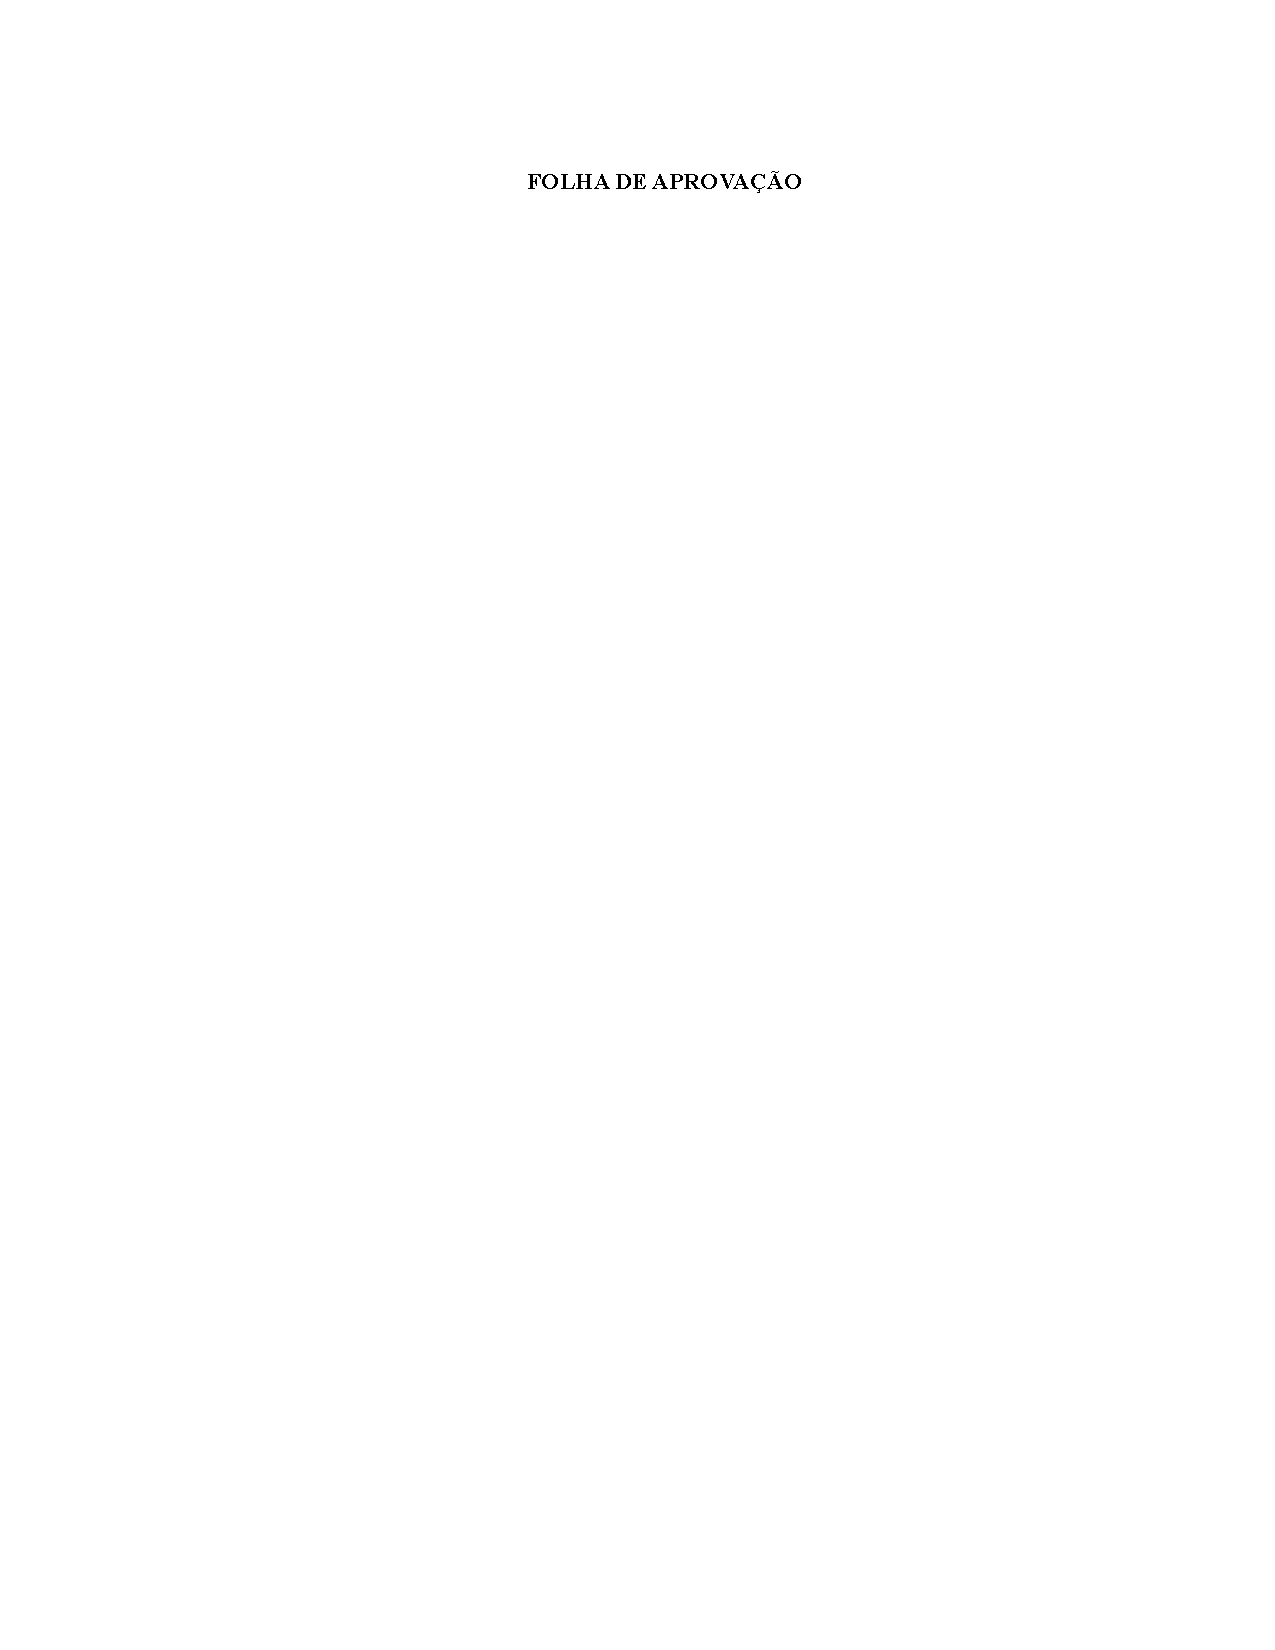
\includepdf[scale=1.0,pages=1]{./PreTexto/folha-aprovacao.pdf} % para adicionar o pdf enviado pelo professor apenas substitua o documento folha-aprovacao.pdf dentro da pasta PreTexto

%% Dedicatória
%%%%% DEDICATÓRIA
%%
%% Texto em que o autor presta homenagem ou dedica seu trabalho.

\begin{dedicatoria}%% Ambiente dedicatoria

    Dedico este trabalho à minha família e amigos, por todo o apoio e suporte durante os altos e baixos desta jornada.

\end{dedicatoria}
%% Comente para remover este item

%% Agradecimentos
%%%%% AGRADECIMENTOS
%%
%% Texto em que o autor faz agradecimentos dirigidos àqueles que contribuíram de maneira relevante à elaboração do trabalho.

\begin{agradecimentos}%% Ambiente agradecimentos

Certamente estas breves palavras não irão atender a todas as pessoas que fizeram parte dessa importante fase de minha vida. Portanto, desde já me desculpo àqueles que não estão presentes entre essas palavras, mas estejam certos que fazem parte do meu pensamento e de minha gratidão. 

Agradeço ao meu orientador Prof. Dr. Prof. Dr. Adolfo Gustavo Serra Seca Neto e ao meu coorientador Prof. Dr. Gustavo Alberto Giménez-Lugo, pela sabedoria com que me guiou nesta trajetória.

Aos meus colegas de sala.

A Secretaria do Curso, pela cooperação.

A todos os professores que me guiaram ao longo do caminho.

Gostaria, também de deixar o meu agradecimento à minha família e amigos, pois acredito que sem o apoio deles seria muito difícil vencer esse desafio. 

Enfim, a todos os que por algum motivo contribuíram para a realização desta pesquisa.


\end{agradecimentos}
%% Comente para remover este item

%% Epígrafe
%%%% EPÍGRAFE
%%
%% Texto em que o autor apresenta uma citação, seguida de indicação de autoria, relacionada com a matéria tratada no corpo do
%% trabalho.

\begin{epigrafe}%% Ambiente epigrafe
Quem construiu Tebas, a cidade das sete portas?
Nos livros estão nomes de reis;
Os reis carregaram as pedras?
E Babilônia, tantas vezes destruída,
Quem a reconstruía sempre?
[...]
Frederico 2º venceu a Guerra dos Sete Anos.
Quem partilhou da vitória?
A cada página uma vitória.
Quem preparava os banquetes?
A cada dez anos um grande homem.
Quem pagava as despesas?
Tantas histórias,
Tantas questões \cite{Brecht1966Perguntas}
\end{epigrafe}
%% Comente para remover este item

%% Resumo
%%%%% RESUMO
%%
%% Apresentação concisa dos pontos relevantes de um texto, fornecendo uma visão rápida e clara do conteúdo e das conclusões do
%% trabalho.

\begin{resumoutfpr}%% Ambiente resumoutfpr
O resumo deve ressaltar de forma sucinta o conteúdo do trabalho, incluindo justificativa, objetivos, metodologia, resultados e conclusão. Deve ser redigido em um único parágrafo, justificado, contendo de 150 até 500 palavras. Evitar incluir citações, fórmulas, equações e símbolos no resumo. A referência no resumo é elemento opcional em trabalhos acadêmicos, sendo que na UTFPR adotamos por não incluí-la nos resumos contidos nos próprios trabalhos. As palavras-chave e as keywords são grafadas em inicial minúscula quando não forem nome próprio ou nome científico e separados por ponto e vírgula.
\end{resumoutfpr}
%% Comente para remover este item

%% Abstract
%%%%% ABSTRACT
%%
%% Versão do resumo para idioma de divulgação internacional.

\begin{abstractutfpr}%% Ambiente abstractutfpr
Seguir o mesmo padrão do resumo, com a tradução do texto do resumo e referência, se houver, para a língua estrangeira (língua inglesa).
\end{abstractutfpr}
%% Comente para remover este item

%% Lista de algoritmos
%\incluirlistadealgoritmos%% Comente para remover este item

%% Lista de ilustrações
%\incluirlistadeilustracoes%% Comente para remover este item

%% Lista de Fotografias
%\incluirlistadefotografias %% Comente para remover este item

%% Lista de Gráficos
%\incluirlistadegraficos %% Comente para remover este item

%% Lista de tabelas
%\incluirlistadetabelas%% Comente para remover este item

%% Lista de quadros
%\incluirlistadequadros

%% Listagem de códigos fonte
%\incluirlistadecodigosfonte

%% Lista de abreviaturas, siglas e acrônimos
%\incluirlistadeacronimos{glossaries}%% Opções: "glossaries" (pacote) ou "file" (arquivo) ou "none" (desabilita)

%% Lista de símbolos
%\incluirlistadesimbolos{nomencl}%% Opções: "nomencl" (pacote) ou "file" (arquivo) ou "none" (desabilita)

%% Sumário
%\incluirsumario%% Comente para remover este item

%% Formatação de páginas de elementos textuais
\textual%% Não comente esta linha

%% Parte
% \part{Introdução}%% Comente para remover este item

%% Capítulo introdução - obrigatório

\chapter{Introdução}\label{cap:introducao}

Neste capítulo pretende-se introduzir brevemente o leitor aos temas pertinentes ao trabalho.
Serão apresentados o tema, seu domínio, objeto e pergunta de pesquisa e 
implicações na computação.
\section{Considerações Iniciais}\label{sec:consideracoes_iniciais}

A indústria de desenvolvimento de software, frequentemente celebrada como um bastião da inovação, criatividade e flexibilidade, opera sobre um paradoxo fundamental. 
Por um lado, 
a concepção e a construção de constructos computacionais são atividades eminentemente intelectuais, que demandam engenhosidade, resolução de problemas complexos e um grau de  
artesanato digital. 
Movimentos como o "\textit{Software Craftsmanship}", Artesanato de Software, surgiram como uma resposta à industrialização do desenvolvimento, enfatizando a 
importância da qualidade, do profissionalismo e do orgulho no trabalho bem-feito, onde o desenvolvedor é visto como um artesão que aprimora suas habilidades e cria produtos de 
alta qualidade.

Por outro lado, esta atividade criativa é, em sua vasta maioria, exercida no interior de estruturas corporativas que aplicam lógicas de produção industrial, buscando 
previsibilidade, padronização e maximização da eficiência. 
Essa abordagem, herdeira da gestão científica de Frederick Taylor, o Taylorismo \cite{Taylor1911}, visa decompor tarefas complexas em 
partes menores e gerenciáveis, otimizar fluxos de trabalho e, idealmente, tornar o trabalhador individual uma peça substituível em uma linha de montagem. 
No desenvolvimento de 
software, isso se manifesta na tentativa de transformar a programação em um processo previsível e mensurável, muitas vezes em detrimento da autonomia e da criatividade do 
engenheiro.

Este trabalho de conclusão de curso se propõe a investigar a tensão inerente a este paradoxo. 
A aplicação de modelos industriais a um trabalho de natureza criativa gera uma 
forma de alienação, conceito analisado por Karl Marx \cite{Marx1844}. 
O trabalhador de software, muitas vezes, encontra-se alienado do produto final de seu trabalho, executando tarefas 
fragmentadas sem uma visão do todo, 
do próprio ato de produção, seguindo processos sobre os quais tem pouco controle, de seus colegas, devido à especialização excessiva, 
e de 
sua própria essência criativa, ao ser reduzido a um executor de tarefas pré-definidas.

Nenhum campo exemplifica melhor essa tensão e suas consequências do que a Inteligência Artificial. 
A IA é o auge da narrativa industrial, a promessa de uma automação completa, 
onde a "inteligência" reside na própria máquina. 
Contudo, essa é uma fachada que oculta uma vasta e diversificada gama de trabalho humano. 
Por trás da aparente autonomia dos 
algoritmos, existe um exército global de "trabalhadores fantasma" (\textit{ghost workers}) \cite{GraySuri2019}, que realizam microtarefas de rotulagem de dados, moderação de conteúdo e correção de erros dos 
sistemas, muitas vezes em condições precárias e por remuneração mínima. 
Esse processo representa a taylorização levada ao extremo, o trabalho cognitivo humano é fragmentado em 
suas unidades mais básicas para "inteligenciar" a máquina, tornando o trabalhador invisível. 

Essa mistificação da IA cumpre uma função ideológica análoga àquela criticada por Álvaro Vieira Pinto \cite{VieiraPinto2005} em sua análise do conceito de "tecno-estrutura" de John K. Galbraith \cite{Galbraith1967}. 
Assim como a ideia de que 
o poder se deslocou do capital para os "técnicos" servia para ocultar a dominação inalterada dos proprietários, a narrativa da "IA inteligente" mascara o poder das corporações 
que detêm os modelos e os dados, e apaga a centralidade do trabalho humano que a constitui. 
A máquina, que na filosofia de Vieira Pinto é um objeto de mediação da ação humana, 
é apresentada como um sujeito autônomo, invertendo a relação fundamental entre criador e criação. 

\section{Domínio}\label{sec:dominio}

Esta pesquisa se situa na interseção entre a Engenharia de Software, a Sociologia do Trabalho e a Teoria Crítica da Tecnologia. 
O domínio abrange a análise dos processos de 
desenvolvimento de software sob a ótica das teorias de organização industrial, como o Taylorismo, e suas críticas, com um foco particular na aplicação desses modelos à produção 
de sistemas de Inteligência Artificial. 
Utiliza-se como referencial teórico a filosofia da tecnologia de Álvaro Vieira Pinto para desmistificar a autonomia da técnica e 
reafirmar a centralidade do sujeito humano, bem como estudos sobre o trabalho digital e o "trabalho fantasma" na economia de plataforma. 

\section{Objeto e Pergunta de Pesquisa}\label{sec:obj_pergunta_pesquisa}

O objeto desta pesquisa é o processo de concepção e produção de constructos computacionais, com ênfase nos sistemas de Inteligência Artificial. 
A investigação se concentra na 
análise do trabalho humano — tanto o trabalho intelectual e criativo dos engenheiros de software quanto o trabalho fragmentado e muitas vezes invisibilizado dos trabalhadores 
de dados, que é sistematicamente ocultado pelos modelos de produção industrial e pelas narrativas de automação que dominam a indústria de tecnologia. 

A partir da tensão exposta, a pergunta que guia esta monografia é: De que maneira os modelos de produção industrial aplicados ao desenvolvimento de software, especialmente na 
área de Inteligência Artificial, geram uma tensão com a natureza criativa do trabalho e resultam no ocultamento do trabalho humano essencial para a sua realização? 

\section{Implicações na Computação}\label{sec:implicacoes_computacao}

As implicações desta pesquisa para a área de Engenharia de Computação são, primordialmente, de ordem crítica e ética. 
Ao desvelar o paradoxo no cerne da produção de software, 
este trabalho desafia a visão puramente técnica e instrumental da engenharia. 
Ele convida os futuros engenheiros a refletirem sobre as seguintes questões: 

\begin{itemize}
    \item \textbf{A Natureza do Trabalho de Engenharia:} Reconhecer a engenharia de software não apenas como uma disciplina técnica, mas como uma prática criativa e intelectual que é impactada e, 
por vezes, limitada por modelos de gestão.
\item \textbf{A Responsabilidade Ética e Social:} Compreender que as escolhas de arquitetura e processo não são neutras. 
Elas estão inseridas em um sistema de produção que tem consequências 
diretas sobre as condições de trabalho de uma vasta cadeia de pessoas, desde os engenheiros na empresa até os trabalhadores de dados em plataformas globais. 
\item \textbf{A Necessidade de uma Prática Crítica:} Incentivar uma postura que questione a finalidade dos sistemas que são construídos e os interesses que eles servem, alinhando-se a uma 
engenharia que, conforme a perspectiva de Vieira Pinto, deve ser centrada no humano e consciente de seu papel como sujeito transformador, e não como mero executor em uma linha 
de montagem industrial. 
\end{itemize}%% Comente para remover este item

%% Capítulo
\chapter{A Concepção do Objeto Técnico}\label{cap:concepcao_obj_tecnico}
 
Este capítulo constrói o alicerce teórico para a análise crítica da concepção de jogos digitais e da Inteligência Artificial, 
conforme proposto na introdução. O objetivo é desmistificar o ato de "conceber um jogo", argumentando que ele transcendeu a criação 
de um mero objeto de entretenimento para se tornar um ato deliberado de engenharia comportamental. A finalidade humana, neste caso, 
a maximização do engajamento e da receita, é inscrita em um objeto técnico que instrumentaliza a psicologia do jogador. A aparente 
"inteligência" dos sistemas de IA que otimizam essa instrumentalização não supera a dialética sujeito-objeto de Álvaro Vieira Pinto \cite{VieiraPinto2005}, 
mas representa sua mais sofisticada forma de ocultamento. Analisaremos como a finalidade corporativa é traduzida em um 
"código comportamental", como esse processo é moldado por relações de poder e, crucialmente, como a narrativa de "jogabilidade 
personalizada" funciona como uma manobra ideológica para obscurecer a intenção manipulativa e o trabalho humano subjacente.

\section{O Trabalho como Fundamento da Técnica e da Hominização}\label{sec:trabalho_como_fundamento}

Para compreender a "concepção de objeto" no contexto tecnológico, é imperativo primeiro estabelecer uma base filosófica que 
transcenda a mera noção de design ou projeto. A concepção de qualquer artefato técnico está fundamentalmente enraizada no conceito 
de trabalho. Na tradição do materialismo histórico, o trabalho não é apenas uma atividade econômica, mas a própria essência da 
atividade humana \cite{Marx2004Manuscritos}, o processo pelo qual o ser humano transforma a natureza para satisfazer suas necessidades e, ao fazê-lo, 
transforma a si mesmo e constrói sua identidade. É através do trabalho que a humanidade se distingue dos outros seres, criando 
cultura, sociedade e história.

Álvaro Vieira Pinto \cite{VieiraPinto2005}, alinhado a essa perspectiva materialista, concebe a técnica não como algo externo ao homem, mas como uma 
extensão dialética de seu próprio ser. A técnica emerge do trabalho como uma mediação entre o homem e a natureza, um prolongamento 
de suas capacidades físicas e intelectuais que permite um domínio crescente sobre o mundo objetivo. Nesta visão, a concepção de um 
objeto técnico não é um ato puramente intelectual ou abstrato, mas uma forma de práxis: a união indissolúvel entre teoria e prática, 
pensamento e ação. Conceber um jogo digital, portanto, não é apenas um exercício de criatividade ou programação,é um ato fundamental 
de trabalho \cite{Marx2004Manuscritos,VieiraPinto2005} que materializa uma intenção humana em um artefato interativo.

\section{A Dialética do Sujeito e do Objeto}\label{sec:dialetica}

Na filosofia da tecnologia de Álvaro Vieira Pinto \cite{VieiraPinto2005}, a dialética entre sujeito e objeto é o ponto de partida para desmistificar a 
tecnologia e situá-la em seu devido lugar, como um produto da existência humana e não como uma força autônoma. O ser humano é o 
único sujeito atuante, um ser histórico dotado de consciência que resolve as contradições de sua existência através do trabalho. 
A máquina, em contrapartida, é, e sempre será, um objeto. Ela é uma mediação, uma extensão da capacidade humana. Vieira Pinto é 
enfático ao afirmar que "a máquina não trabalha". Ela pode executar efeitos dinâmicos, mas o faz como um instrumento passivo, 
seguindo o programa que lhe foi "embutido pelo seu criador, o cérebro humano".

A aplicação direta desta dialética à Inteligência Artificial nos jogos é fundamental. A "inteligência" de um algoritmo de 
\textit{matchmaking} ou de um sistema de precificação dinâmica não é uma propriedade intrínseca do objeto, mas a "exteriorização e a 
multiplicação da racionalidade do sujeito que o concebeu" \cite{VieiraPinto2005}. O discurso corporativo, no entanto, frequentemente inverte essa relação, 
usando frases como "o algoritmo decidiu pareá-lo com este oponente" ou "o sistema personalizou esta oferta para você". Essa inversão 
não é um erro linguístico inocente, é o primeiro passo de uma sofisticada mistificação ideológica. Ao antropomorfizar o objeto, 
esvazia-se a responsabilidade do sujeito humano, o engenheiro, o designer de monetização, a corporação. Se o algoritmo é o sujeito 
que "decide", então o criador humano é absolvido da responsabilidade pelas consequências dessa decisão, seja uma experiência de jogo 
frustrante projetada para induzir gastos ou uma oferta predatória direcionada a um jogador vulnerável. A própria linguagem usada para 
descrever a IA nos jogos torna-se um campo de batalha ideológico, preparando o terreno para o ocultamento do poder e da intenção por 
trás do sistema.

\section{A Natureza do Objeto Técnico}\label{sec:natureza_obj_tec}

A visão comum da tecnologia tende a reduzi-la a um conjunto de ferramentas neutras. A Teoria Crítica da Tecnologia de Andrew Feenberg \cite{Feenberg1999}
desafia essa concepção, argumentando que a tecnologia nunca é neutra, ela é um palco de valores sociais e políticos. Todo artefato 
técnico possui um "código técnico", um conjunto de regras e pressupostos embutidos em seu design que refletem e reforçam uma 
determinada visão de mundo e específicas relações de poder \cite{Feenberg2002Transforming}. A escolha de design entre múltiplas possibilidades tecnicamente viáveis é 
sempre política.

No contexto dos jogos digitais potencializados por IA, esse conceito pode ser aprofundado. Conforme argumentam Jong e Prey \cite{deJongPrey2022}, o código 
técnico de muitos sistemas algorítmicos contemporâneos é, fundamentalmente, o Behaviorismo. Esta é uma visão de mundo que reduz o ser 
humano a um conjunto de comportamentos observáveis, previsíveis e controláveis, ignorando a complexidade da subjetividade. Este 
trabalho postula que o código técnico dos sistemas de IA em jogos digitais é, precisamente, um "código comportamental". Os algoritmos 
de monetização e engajamento não são neutros, eles codificam uma visão empobrecida e instrumental do ser humano, tratando o jogador 
não como um sujeito a ser entretido, mas como um sistema de respostas a ser otimizado para a extração de valor. A engenharia de 
software, neste contexto, transcende a construção de funcionalidades para se tornar a codificação de uma epistemologia behaviorista 
que serve a fins comerciais.

\section{A Inscrição da Finalidade Comercial no Código Comportamental}\label{sec:inscricao_finalidade}

Em sistemas de IA, a inscrição da finalidade assume uma forma diferente da programação tradicional. Ela se materializa como a 
arquitetura de um vasto espaço de possibilidades, moldado pelos dados de treinamento e pelos objetivos de otimização. Nos jogos 
digitais, o ato de "conceber" um sistema de monetização com IA e de lhe atribuir a finalidade de "maximizar a receita" torna-se o ato 
de projetar um sistema que aprende e se adapta para explorar a psicologia do jogador.

A finalidade comercial é inscrita através de:

\begin{itemize}
    \item \textbf{Testes A/B em Larga Escala:} Sistemas de IA podem executar milhares de testes simultaneamente, variando preços, ofertas e a 
    apresentação visual de itens para diferentes segmentos de jogadores \cite{Lupianez-Villanueva2022}, identificando e aplicando automaticamente as táticas que 
    geram maior conversão. 
    
    \item \textbf{Precificação Dinâmica:} Algoritmos analisam o histórico de compras, o tempo de jogo e outros dados comportamentais de um 
    jogador para calcular o preço máximo que ele estaria disposto a pagar por um item e apresentar uma oferta "personalizada" nesse 
    exato valor.
    
    \item \textbf{Geração Procedural de Conteúdo para Retenção:} A IA pode gerar desafios, missões ou mapas adaptados ao nível de habilidade 
    do jogador, não para maximizar a diversão, mas para mantê-lo em um estado de engajamento ótimo que o torne mais propenso a gastar.
\end{itemize}

A natureza estatística e opaca desses sistemas, o chamado "problema da caixa-preta", é uma poderosa ferramenta ideológica. Ela 
permite que decisões de design manipulativas sejam apresentadas como resultados "otimizados" e "emergentes" do processo de 
aprendizado da máquina \cite{Bender2021}, em vez de escolhas deliberadas de seus criadores. A ideologia da extração de valor é, assim, "lavada" através 
da estatística, transformando decisões de negócio em resultados aparentemente neutros e técnicos.

\section{A Concepção como Arena Sociopolítica}\label{sec:concepcao_arena_sociopolitica}

A concepção de um jogo não ocorre em um vácuo. Ela está imersa em contextos sociais e políticos que moldam sua forma e função. A 
teoria da Construção Social da Tecnologia, \textit{SCOT} \cite{BijkerPinch1989} argumenta que o design é negociado por diferentes "grupos sociais relevantes". 
Na indústria de jogos, esses grupos incluem não apenas desenvolvedores e jogadores, mas também executivos, investidores, equipes de 
marketing e, cada vez mais, especialistas como \textit{game economists} e designers de monetização.

A finalidade inscrita nos jogos reflete os interesses do grupo dominante, o capital. A pressão corporativa por metas de receita 
trimestrais impulsiona a adoção de mecânicas de monetização agressivas e \textit{dark patterns}, mesmo que prejudiquem a experiência 
do jogador a longo prazo \cite{PetrovskayaZendle2022}. O designer ou engenheiro, neste contexto, muitas vezes atua não como um criador autônomo, mas como um 
trabalhador cuja criatividade é direcionada para resolver o problema de "como extrair mais valor do jogador". Este processo depende 
de uma cadeia global de trabalho, desde os desenvolvedores em regime de \textit{crunch} até os testadores precarizados, cujo trabalho 
coletivo para criar o jogo é sistematicamente ocultado por trás da marca do estúdio.

\section{A Mistificação do Objeto}\label{sec:mistificacao_obj}

A crítica de Álvaro Vieira Pinto ao conceito de "tecno-estrutura" de Galbraith \cite{VieiraPinto2005,Galbraith1967} oferece um análogo preciso para compreender a 
mistificação contemporânea da IA nos jogos. Galbraith argumentava que o poder havia se deslocado do capital para os "técnicos". 
Vieira Pinto desmonta essa noção, mostrando que o conhecimento técnico é apenas uma mercadoria comprada pelo capital, e a 
"tecno-estrutura" é uma fachada ideológica para mascarar a dominação inalterada dos proprietários.

A narrativa do jogo "inteligente" ou "adaptativo" desempenha a mesma função. Ao atribuir agência ao sistema de IA, que "aprende" o 
comportamento do jogador e "personaliza" a experiência, desvia-se a atenção dos verdadeiros agentes, as corporações que detêm os 
modelos e os dados, e que os controlam para fins de lucro. A IA torna-se a nova tecno-estrutura, uma fachada de objetividade técnica 
que oculta as relações de produção e a finalidade de manipulação. Essa mistificação torna invisível tanto o trabalho precarizado que 
constrói o jogo \cite{GraySuri2019} quanto a intenção deliberada de engenharia comportamental que o anima, transformando uma relação de exploração 
econômica em uma "funcionalidade" de software.

\section{A Reafirmação da Agência Humana na Lei e no Trabalho}\label{sec:reafirmacao_agencia_humana}

A crescente sofisticação dos sistemas de IA em jogos, alimentada pelo discurso de sua autonomia, provocou uma reação social e 
institucional que busca reafirmar a centralidade e a responsabilidade humanas. Este movimento contesta na prática a mistificação do 
objeto.

Na esfera regulatória, o \textit{Al Act} da União Europeia \cite{EU_AI_Act2024}, que proíbe o uso de "técnicas subliminares que ultrapassem a consciência 
de uma pessoa" para manipular o comportamento , e decisões como a da Autoridade Holandesa para Consumidores e Mercados, a \textit{ACM} 
contra a \textit{Epic Games} \cite{ACM2024EpicGames}, são exemplos claros. A multa à \textit{Epic} por usar \textit{dark patterns} como temporizadores de 
contagem regressiva falsos em \textit{Fortnite} não penalizou um algoritmo autônomo, mas responsabilizou a empresa humana por suas 
escolhas de design predatórias, especialmente contra crianças. Essas ações forçam legalmente o restabelecimento do ser humano como o 
sujeito soberano e a IA como o objeto que serve aos seus propósitos \cite{EU_AI_Act2024}.

No campo do trabalho, a greve da \textit{Writers Guild of America - WGA} em 2023, que garantiu que a IA não pudesse ser creditada 
como "escritora" \cite{WGA_MBA2023} , ecoa as preocupações da indústria de jogos. A luta é para que a concepção da obra, seja um roteiro ou um jogo, 
permaneça uma prerrogativa humana, relegando a IA à sua posição correta de ferramenta. Essas lutas regulatórias e trabalhistas são a 
prova de que a dialética sujeito-objeto é o cerne da política tecnológica contemporânea, forçando a reafirmação da agência e da 
responsabilidade humana contra a narrativa de autonomia da máquina.

\section{Consciência Crítica na Concepção}\label{sec:consciencia_critica_concepcao}

A análise desenvolvida neste capítulo demonstra que a concepção de um jogo digital potencializado por IA, longe de ser um processo 
técnico neutro, é um ato profundamente humano, social e político. A partir do referencial de Álvaro Vieira Pinto \cite{VieiraPinto2005}, foi estabelecido 
que a relação fundamental é a de um sujeito que cria um objeto de mediação para satisfazer uma finalidade. Nos jogos modernos, essa 
finalidade é crescentemente a extração de valor, inscrita em um "código comportamental" \cite{deJongPrey2022} que visa modular a psicologia do jogador.

A narrativa de autonomia da IA foi desmistificada como uma fachada ideológica que oculta o poder corporativo e o trabalho humano \cite{VieiraPinto2005}. As 
implicações para a engenharia são profundas. Uma prática de engenharia consciente não pode se esconder atrás da suposta objetividade 
do artefato. Ela deve reconhecer sua posição como agente no processo de concepção, questionando as finalidades impostas e assumindo 
a responsabilidade pela mediação que seus objetos criam no mundo. A verdadeira "inteligência" não reside no artefato, mas na 
consciência crítica do sujeito que o concebe e na coletividade de sujeitos cujo trabalho o torna possível. Alinhar-se a uma 
engenharia centrada no humano significa assumir o papel de sujeito transformador, e não o de mero executor em uma linha de montagem 
industrial digital.

%% Comente para remover este item

%% Capítulo
%\chapter{A Concepção na Indústria de Criação e Manipulação de Constructos Computacionais}\label{cap:concepcao_industria}

- Exemplificar alguns processos de industrialização e concepção de Constructos Computacionais(Modelos Computacionais, Softwares, etc)%% Comente para remover este item

%% Capítulo
%\chapter{Materiais e Métodos}\label{cap:materiais_metodos}

- Apresentar como será trabalhado o projeto citando materiais usados e os métodos adotados para o desenvolvimento deste%% Comente para remover este item

%% Capítulo
%\chapter{Ainda sem nome}\label{cap:cap5}

- Resgatar um dos exemplos de processos de industrialização e concepção de constructos do capitulo 3 e se aprofundar neste mostrando como há pontos em que colaboradores essenciais para o processo são muitas vezes ocultos e/ou ignorados.%% Comente para remover este item

%% Capítulo
%\chapter{ Análise e Desdobramentos do Capitulo 5(processo)}\label{cap:cap6}

- Partindo do aprofundamento feito no capitulo 5, analisar e propor mudanças ao processo abordado no capitulo 5 de modo que toda e qualquer colaboração significante seja creditada, não somente as mais prestigiosas ou centrais.%% Comente para remover este item

%% Capítulo
%\chapter{Conclusões e Trabalhos Futuros}\label{cap:conclusoes}

%% Comente para remover este item

%% Capítulos após este comando criam marcadores do pdf na raiz
% \phantompart%% Comente para remover este item


%% Formatação de páginas de elementos pós-textuais
\postextual%% Não comente esta linha

%% Arquivos de referências
\arquivosdereferencias{%% Arquivos bibtex sem a extensão .bib e separados por vírgula - Não comente esta linha
  %./PosTexto/exemplos-referencias,%% Arquivo de referências - Comente para remover este item
  main%% Arquivo de referências - Comente para remover este item
}%% Não comente esta linha

%% Glossário
%\incluirglossario %% Comente para remover este item

%% Arquivos de apêndices
 \begin{arquivosdeapendices}%% Os arquivos de apêndices devem se incluídos neste ambiente - Não comente esta linha
%   %\partapendices%% Página de início dos apêndices - adiciona uma página com o título Apêndices
%   %% Capítulo de exemplo
   %%%%% APÊNDICE A
%%
%% Texto ou documento elaborado pelo autor, a fim de complementar sua argumentação, sem prejuízo da unidade nuclear do trabalho.

%% Título e rótulo de apêndice (rótulos não devem conter caracteres especiais, acentuados ou cedilha)
\chapter{Título do Apêndice A com um Texto Muito Longo que Pode Ocupar Mais de uma Linha}\label{cap:apendicea}

Quando houver necessidade pode-se apresentar como apêndice documento(s) auxiliar(es) e/ou complementar(es) como: legislação, estatutos, gráficos, tabelas, etc. Os apêndices são enumerados com letras maiúsculas: \autoref{cap:apendicea}, \autoref{cap:apendiceb}, etc.

No \latex\ apêndices são editados como capítulos. O comando \verb|\appendix| faz com que todos os capítulos seguintes sejam considerados apêndices.

Apêndices complementam o texto principal da tese com informações para leitores com especial interesse no tema, devendo ser considerados leitura opcional, ou seja, o entendimento do texto principal da tese não deve exigir a leitura atenta dos apêndices.

Apêndices usualmente contemplam provas de teoremas, deduções de fórmulas matemáticas, diagramas esquemáticos, gráficos e trechos de código. Quanto a este último, código extenso não deve fazer parte da tese, mesmo como apêndice. O ideal é disponibilizar o código na Internet para os interessados em examiná-lo ou utilizá-lo.

%% Título e rótulo de seção (rótulos não devem conter caracteres especiais, acentuados ou cedilha)
%\section{Título da Seção Secundária do Apêndice B}\label{sec:secaoapendicea}

%Exemplo de seção secundária em apêndice (\autoref{sec:secaoapendicea} do \autoref{cap:apendicea}).

%% Título e rótulo de seção (rótulos não devem conter caracteres especiais, acentuados ou cedilha)
%\subsection{Título da Seção Terciária do Apêndice B}\label{subsec:subsecaoapendicea}

%Exemplo de seção terciária em apêndice (\autoref{subsec:subsecaoapendicea} do \autoref{cap:apendicea}).

%% Título e rótulo de seção (rótulos não devem conter caracteres especiais, acentuados ou cedilha)
%\subsubsection{Título da seção quaternária do Apêndice B}\label{subsubsec:subsubsecaoapendicea}

%Exemplo de seção quaternária em apêndice (\autoref{subsubsec:subsubsecaoapendicea} do \autoref{cap:apendicea}).

%% Título e rótulo de seção (rótulos não devem conter caracteres especiais, acentuados ou cedilha)
%\paragraph{Título da seção quinária do Apêndice B}\label{para:paragraphapendicea}

%Exemplo de seção quinária em apêndice (\autoref{para:paragraphapendicea} do \autoref{cap:apendicea}).
%% Apêndice - Comente para remover este item
   %%%%% APÊNDICE B
%%
%% Texto ou documento elaborado pelo autor, a fim de complementar sua argumentação, sem prejuízo da unidade nuclear do trabalho.

%% Título e rótulo de apêndice (rótulos não devem conter caracteres especiais, acentuados ou cedilha)
\chapter{Orçamentos dos Materiais para Montagem da Bancada Experimental}\label{cap:apendiceb}

\begin{table}[htb]%% Ambiente table
\caption{Orçamento dos materiais n.\textsuperscript{o} 1.}%% Legenda
\label{tab:tab3}%% Rótulo
\begin{tabularx}{\textwidth}{@{\extracolsep{\fill}}lrrr}%% Ambiente tabularx
\toprule
Material              & \multicolumn{1}{c}{Valor (R\$)} & \multicolumn{1}{c}{Quantidade}  & \multicolumn{1}{c}{Total (R\$)} \\ \midrule
Bomba centrífuga      & 2500,00                         & 01                              & 2500,00                         \\
Compressor rotativo   & 3000,00                         & 01                              & 3000,00                         \\
Manômetro diferencial & 450,00                          & 02                              & 900,00                          \\
Termopar              & 370,00                          & 02                              & 740,00                          \\
Válvula de esfera     & 43,00                           & 02                              & 86,00                           \\
Tubulação de PVC      & 10,00                           & 05                              & 50,00                           \\
Conexão de PVC        & 5,00                            & 10                              & 50,00                           \\ \midrule
                      &                                 & \multicolumn{1}{r}{Total (R\$)} & 7326,00                         \\ \bottomrule
\end{tabularx}
\fonte{}%% Fonte
\end{table}

\begin{table}[htb]%% Ambiente table
\caption{Orçamento dos materiais n.\textsuperscript{o} 2.}%% Legenda
\label{tab:tab4}%% Rótulo
\begin{tabularx}{\textwidth}{@{\extracolsep{\fill}}lrrr}%% Ambiente tabularx
\toprule
Material              & \multicolumn{1}{c}{Valor (R\$)} & \multicolumn{1}{c}{Quantidade}  & \multicolumn{1}{c}{Total (R\$)} \\ \midrule
Bomba centrífuga      & 2700,00                         & 01                              & 2700,00                         \\
Compressor rotativo   & 2950,00                         & 01                              & 2950,00                         \\
Manômetro diferencial & 515,00                          & 02                              & 1030,00                         \\
Termopar              & 350,00                          & 02                              & 700,00                          \\
Válvula de esfera     & 40,00                           & 02                              & 80,00                           \\
Tubulação de PVC      & 8,00                            & 05                              & 40,00                           \\
Conexão de PVC        & 6,00                            & 10                              & 60,00                           \\ \midrule
                      &                                 & \multicolumn{1}{r}{Total (R\$)} & 7560,00                         \\ \bottomrule
\end{tabularx}
\fonte{}%% Fonte
\end{table}

\begin{table}[htb]%% Ambiente table
\caption{Orçamento dos materiais n.\textsuperscript{o} 3.}%% Legenda
\label{tab:tab5}%% Rótulo
\begin{tabularx}{\textwidth}{@{\extracolsep{\fill}}lrrr}%% Ambiente tabularx
\toprule
Material              & \multicolumn{1}{c}{Valor (R\$)} & \multicolumn{1}{c}{Quantidade}  & \multicolumn{1}{c}{Total (R\$)} \\ \midrule
Bomba centrífuga      & 2600,00                         & 01                              & 2600,00                         \\
Compressor rotativo   & 3100,00                         & 01                              & 3100,00                         \\
Manômetro diferencial & 500,00                          & 02                              & 1000,00                         \\
Termopar              & 400,00                          & 02                              & 800,00                          \\
Válvula de esfera     & 45,00                           & 02                              & 90,00                           \\
Tubulação de PVC      & 12,00                           & 05                              & 60,00                           \\
Conexão de PVC        & 5,00                            & 10                              & 50,00                           \\ \midrule
                      &                                 & \multicolumn{1}{r}{Total (R\$)} & 7700,00                         \\ \bottomrule
\end{tabularx}
\fonte{}%% Fonte
\end{table}
%% Apêndice - Comente para remover este item
 \end{arquivosdeapendices}%% Não comente esta linha


% \begin{apendicesenv}%% Ambiente apendicesenv

% \partapendices
% \chapter{Ola}

% \lipsum[55-56]

% \end{apendicesenv}

%% Arquivos de anexos
\begin{arquivosdeanexos}%% Os arquivos de anexos devem se incluídos neste ambiente - Não comente esta linha
  %\partanexos%% Página de início dos anexos - adiciona uma página com o título Anexos

  %%%%% ANEXO A
%%
%% Texto ou documento não elaborado pelo autor, que serve de fundamentação, comprovação e ilustração.

%% Título e rótulo de anexo (rótulos não devem conter caracteres especiais, acentuados ou cedilha)
\anexos
\chapter{Direitos Autorais - Lei N\texorpdfstring{.\textsuperscript{o}}{o.} 9.610, de 19 de Fevereiro de 1998: Disposições Preliminares}\label{cap:anexoa}

\centerline{\includegraphics[width=\textwidth]{./PosTexto/Ilustracoes/lei-n9610-p1}}%% Imagem (Dimensões e localização)

\centerline{\includegraphics[width=\textwidth]{./PosTexto/Ilustracoes/lei-n9610-p2}}%% Imagem (Dimensões e localização)
%% Anexo - Comente para remover este item
  %%%%% ANEXO B
%%
%% Texto ou documento não elaborado pelo autor, que serve de fundamentação, comprovação e ilustração.

%% Título e rótulo de anexo (rótulos não devem conter caracteres especiais, acentuados ou cedilha)
\chapter{Normas para Elaboração de Trabalhos Acadêmicos}\label{cap:anexob}

As normas da \gls{utfpr} podem ser acessadas em: \url{http://portal.utfpr.edu.br/biblioteca/trabalhos-academicos/discentes/orientacao-para-trabalhos-academicos}. Ver Figura \ref{fig:capadolivro}.

\begin{figure}[htb]%% Ambiente figure
\captionsetup{width=0.9\textwidth}%% Largura da legenda
\caption{Sítio: Normas para Elaboração de Trabalhos Acadêmicos.}%% Legenda
\label{fig:capadolivro}%% Rótulo
\includegraphics[width=0.9\textwidth]{normas}%% Dimensões e localização
\fonte{\cite{UTFPR2008}}%% Fonte
\end{figure}

%% Anexo - Comente para remover este item
\end{arquivosdeanexos}%% Não comente esta linha

%% Índice - Adiciona um índice remissivo.
%\incluirindice%% Comente para remover este item

%% Fim do documento
\end{document}%% Não comente esta linha
